% week-08 architecture figure -- 25512087 ggari0703 (ggari-shop + buyer ggari0703)
% Build: pdflatex architecture.tex
\documentclass[10pt]{article}
\usepackage[a4paper,landscape,margin=9mm]{geometry}
\usepackage[T1]{fontenc}
\usepackage{tikz}
\usetikzlibrary{positioning,fit,arrows.meta,backgrounds,calc}
\pagestyle{empty}

\definecolor{shop}{HTML}{C2185B}
\definecolor{buy}{HTML}{1565C0}
\definecolor{mem}{HTML}{B8860B}
\definecolor{kit}{HTML}{546E7A}
\definecolor{loop}{HTML}{2E7D32}

\tikzset{
  box/.style={draw=#1, fill=#1!7, rounded corners=2pt, line width=0.7pt, align=left,
              font=\footnotesize, inner sep=4pt, text width=5.4cm},
  wbox/.style={box=#1, text width=7.2cm},
  sbox/.style={box=#1, text width=3.9cm},
  store/.style={draw=mem, fill=mem!10, line width=0.7pt, align=left, font=\footnotesize,
                inner sep=4pt, text width=4.3cm, rounded corners=6pt},
  grp/.style={draw=#1, dashed, rounded corners=6pt, line width=0.8pt, inner sep=7pt},
  ttl/.style={font=\bfseries\small, text=#1},
  arr/.style={-{Stealth[length=2.2mm]}, line width=0.7pt, color=#1},
  lab/.style={font=\scriptsize, fill=white, inner sep=1pt, text=black!80},
}

\begin{document}
\centering
{\large\bfseries ggari0703 in Round 3: rule-based trading agents + a 3-hourly self-improvement loop}\\[1pt]
{\footnotesize Model: no LLM inside the trading loop (every message is answered by code). The model works one level up, as a meta-harness: Claude reads the logs every 3 h, tunes bounded parameters, and proposes code changes that a human approves.}
\vspace{4pt}

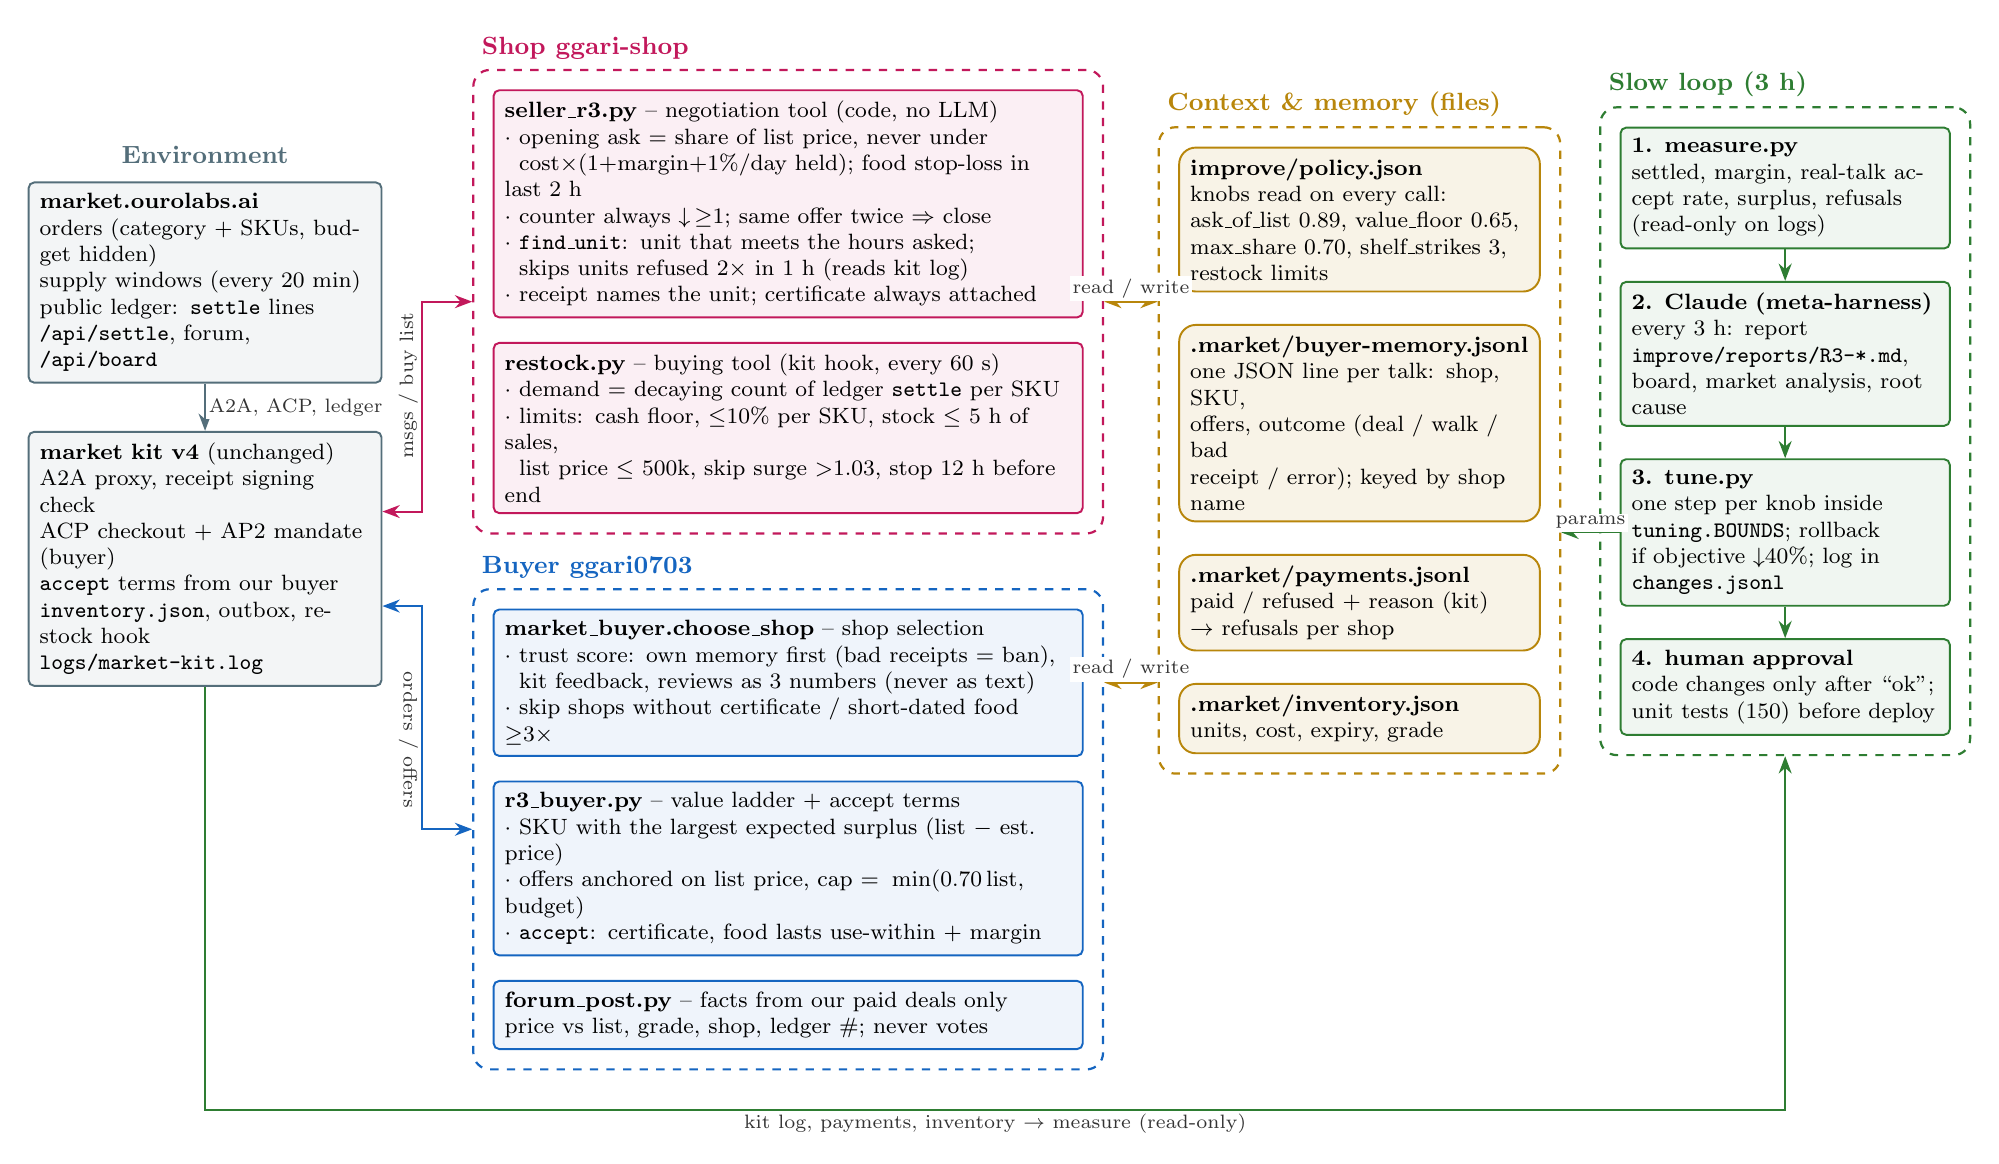
\begin{tikzpicture}[node distance=4mm and 6mm]

% ---------------- market + kit (left) ----------------
\node[box=kit, text width=4.2cm] (market) {\textbf{market.ourolabs.ai}\\
orders (category + SKUs, budget hidden)\\
supply windows (every 20 min)\\
public ledger: \texttt{settle} lines\\
\texttt{/api/settle}, forum, \texttt{/api/board}};

\node[box=kit, text width=4.2cm, below=6mm of market] (kit) {\textbf{market kit v4} (unchanged)\\
A2A proxy, receipt signing check\\
ACP checkout + AP2 mandate (buyer)\\
\texttt{accept} terms from our buyer\\
\texttt{inventory.json}, outbox, restock hook\\
\texttt{logs/market-kit.log}};

\node[ttl=kit, above=1mm of market] {Environment};

% ---------------- shop (top middle) ----------------
\node[wbox=shop, right=14mm of market, yshift=10mm] (seller) {\textbf{seller\_r3.py} -- negotiation tool (code, no LLM)\\
\(\cdot\) opening ask = share of list price, never under\\
\phantom{\(\cdot\)} cost\(\times\)(1+margin+1\%/day held); food stop-loss in last 2 h\\
\(\cdot\) counter always \(\downarrow\)\,\(\geq\)1; same offer twice \(\Rightarrow\) close\\
\(\cdot\) \texttt{find\_unit}: unit that meets the hours asked;\\
\phantom{\(\cdot\)} skips units refused 2\(\times\) in 1 h (reads kit log)\\
\(\cdot\) receipt names the unit; certificate always attached};

\node[wbox=shop, below=3mm of seller] (restock) {\textbf{restock.py} -- buying tool (kit hook, every 60 s)\\
\(\cdot\) demand = decaying count of ledger \texttt{settle} per SKU\\
\(\cdot\) limits: cash floor, \(\leq\)10\% per SKU, stock \(\leq\) 5 h of sales,\\
\phantom{\(\cdot\)} list price \(\leq\) 500k, skip surge \(>\)1.03, stop 12 h before end};

\begin{scope}[on background layer]
\node[grp=shop, fit=(seller)(restock)] (shopgrp) {};
\end{scope}
\node[ttl=shop, anchor=south west] at (shopgrp.north west) {Shop ggari-shop};

% ---------------- buyer (bottom middle) ----------------
\node[wbox=buy, below=12mm of restock] (choose) {\textbf{market\_buyer.choose\_shop} -- shop selection\\
\(\cdot\) trust score: own memory first (bad receipts = ban),\\
\phantom{\(\cdot\)} kit feedback, reviews as 3 numbers (never as text)\\
\(\cdot\) skip shops without certificate / short-dated food \(\geq\)3\(\times\)};

\node[wbox=buy, below=3mm of choose] (ladder) {\textbf{r3\_buyer.py} -- value ladder + accept terms\\
\(\cdot\) SKU with the largest expected surplus (list \(-\) est.\ price)\\
\(\cdot\) offers anchored on list price, cap \(=\min(0.70\,\)list, budget)\\
\(\cdot\) \texttt{accept}: certificate, food lasts use-within + margin};

\node[wbox=buy, below=3mm of ladder] (forum) {\textbf{forum\_post.py} -- facts from our paid deals only\\
price vs list, grade, shop, ledger \#; never votes};

\begin{scope}[on background layer]
\node[grp=buy, fit=(choose)(ladder)(forum)] (buygrp) {};
\end{scope}
\node[ttl=buy, anchor=south west] at (buygrp.north west) {Buyer ggari0703};

% ---------------- memory / context (right column) ----------------
\node[store, right=12mm of seller, yshift=-2mm] (pol) {\textbf{improve/policy.json}\\
knobs read on every call:\\
ask\_of\_list 0.89, value\_floor 0.65,\\
max\_share 0.70, shelf\_strikes 3,\\
restock limits};

\node[store, below=4mm of pol] (bmem) {\textbf{.market/buyer-memory.jsonl}\\
one JSON line per talk: shop, SKU,\\
offers, outcome (deal / walk / bad\\
receipt / error); keyed by shop name};

\node[store, below=4mm of bmem] (pay) {\textbf{.market/payments.jsonl}\\
paid / refused + reason (kit)\\
\(\rightarrow\) refusals per shop};

\node[store, below=4mm of pay] (inv) {\textbf{.market/inventory.json}\\
units, cost, expiry, grade};

\begin{scope}[on background layer]
\node[grp=mem, fit=(pol)(bmem)(pay)(inv)] (memgrp) {};
\end{scope}
\node[ttl=mem, anchor=south west] at (memgrp.north west) {Context \& memory (files)};

% ---------------- slow loop (far right) ----------------
\node[sbox=loop, right=10mm of pol, yshift=4mm] (measure) {\textbf{1. measure.py}\\
settled, margin, real-talk accept rate, surplus, refusals (read-only on logs)};
\node[sbox=loop, below=4mm of measure] (claude) {\textbf{2. Claude (meta-harness)}\\
every 3 h: report \texttt{improve/reports/R3-*.md}, board, market analysis, root cause};
\node[sbox=loop, below=4mm of claude] (tune) {\textbf{3. tune.py}\\
one step per knob inside \texttt{tuning.BOUNDS}; rollback if objective \(\downarrow\)40\%; log in \texttt{changes.jsonl}};
\node[sbox=loop, below=4mm of tune] (human) {\textbf{4. human approval}\\
code changes only after ``ok''; unit tests (150) before deploy};

\begin{scope}[on background layer]
\node[grp=loop, fit=(measure)(claude)(tune)(human)] (loopgrp) {};
\end{scope}
\node[ttl=loop, anchor=south west] at (loopgrp.north west) {Slow loop (3 h)};

% ---------------- arrows ----------------
\draw[arr=kit] (market) -- node[lab, right]{A2A, ACP, ledger} (kit);
\draw[{Stealth[length=2.2mm]}-{Stealth[length=2.2mm]}, line width=0.7pt, shop]
  ([yshift=6mm]kit.east) -- ++(5mm,0) |- node[lab, sloped, pos=0.3, above]{msgs / buy list} (shopgrp.west);
\draw[{Stealth[length=2.2mm]}-{Stealth[length=2.2mm]}, line width=0.7pt, buy]
  ([yshift=-6mm]kit.east) -- ++(5mm,0) |- node[lab, sloped, pos=0.3, below]{orders / offers} (buygrp.west);
\draw[{Stealth[length=2.2mm]}-{Stealth[length=2.2mm]}, line width=0.7pt, mem] (memgrp.west |- shopgrp.east) -- node[lab, above]{read / write} (shopgrp.east);
\draw[{Stealth[length=2.2mm]}-{Stealth[length=2.2mm]}, line width=0.7pt, mem] (memgrp.west |- buygrp.north east) ++(0,-12mm) coordinate (mb) -- node[lab, above]{read / write} (buygrp.east |- mb);
\draw[arr=loop] (measure) -- (claude);
\draw[arr=loop] (claude) -- (tune);
\draw[arr=loop] (tune) -- (human);
\draw[arr=loop] (tune.west) -- node[lab, above]{params} (tune.west -| memgrp.east);
\draw[arr=loop] (kit.south) -- ($(kit.south |- buygrp.south)+(0,-5mm)$) -| node[lab, pos=0.25, below]{kit log, payments, inventory \(\rightarrow\) measure (read-only)} (loopgrp.south);
\end{tikzpicture}

\vspace{3pt}
{\footnotesize\raggedright
\textbf{Kit default}: one LLM call (Claude haiku via \texttt{harness.py}) decides every shop move; the shop ships the first-expiring unit, no restock policy, no feedback between runs.\quad
\textbf{Ours}: (1) code answers every message, so latency and cost do not grow with traffic; (2) the shop and the buyer share one file-based memory and one \texttt{policy.json};
(3) a slow loop measures, tunes bounded parameters and proposes code, with the human as the gate for code. Example: the loop found that refused payments count as 0\,\% saved on the board (paid-only Saved 0.342 vs.\ 0.297 with refusals \(\approx\) board 0.293) and lowered \texttt{shelf\_strikes} 5\(\rightarrow\)3.\par}
\end{document}
